\section{Methods}

In order to demonstrate that the DISHTINY platform selects for detectable hierarchical transitions in individuality, we performed experiments where cells controlled by evolving genetic programs evolved open-ended behaviors to make decisions about resource sharing, reproductive timing, and apoptosis.
We will first cover the design of the DISHTINY platform and then describe the cell-like organisms we used to evaluate the platform.

\subsection{Resource Collection}

\begin{figure*}[t]
\begin{center}
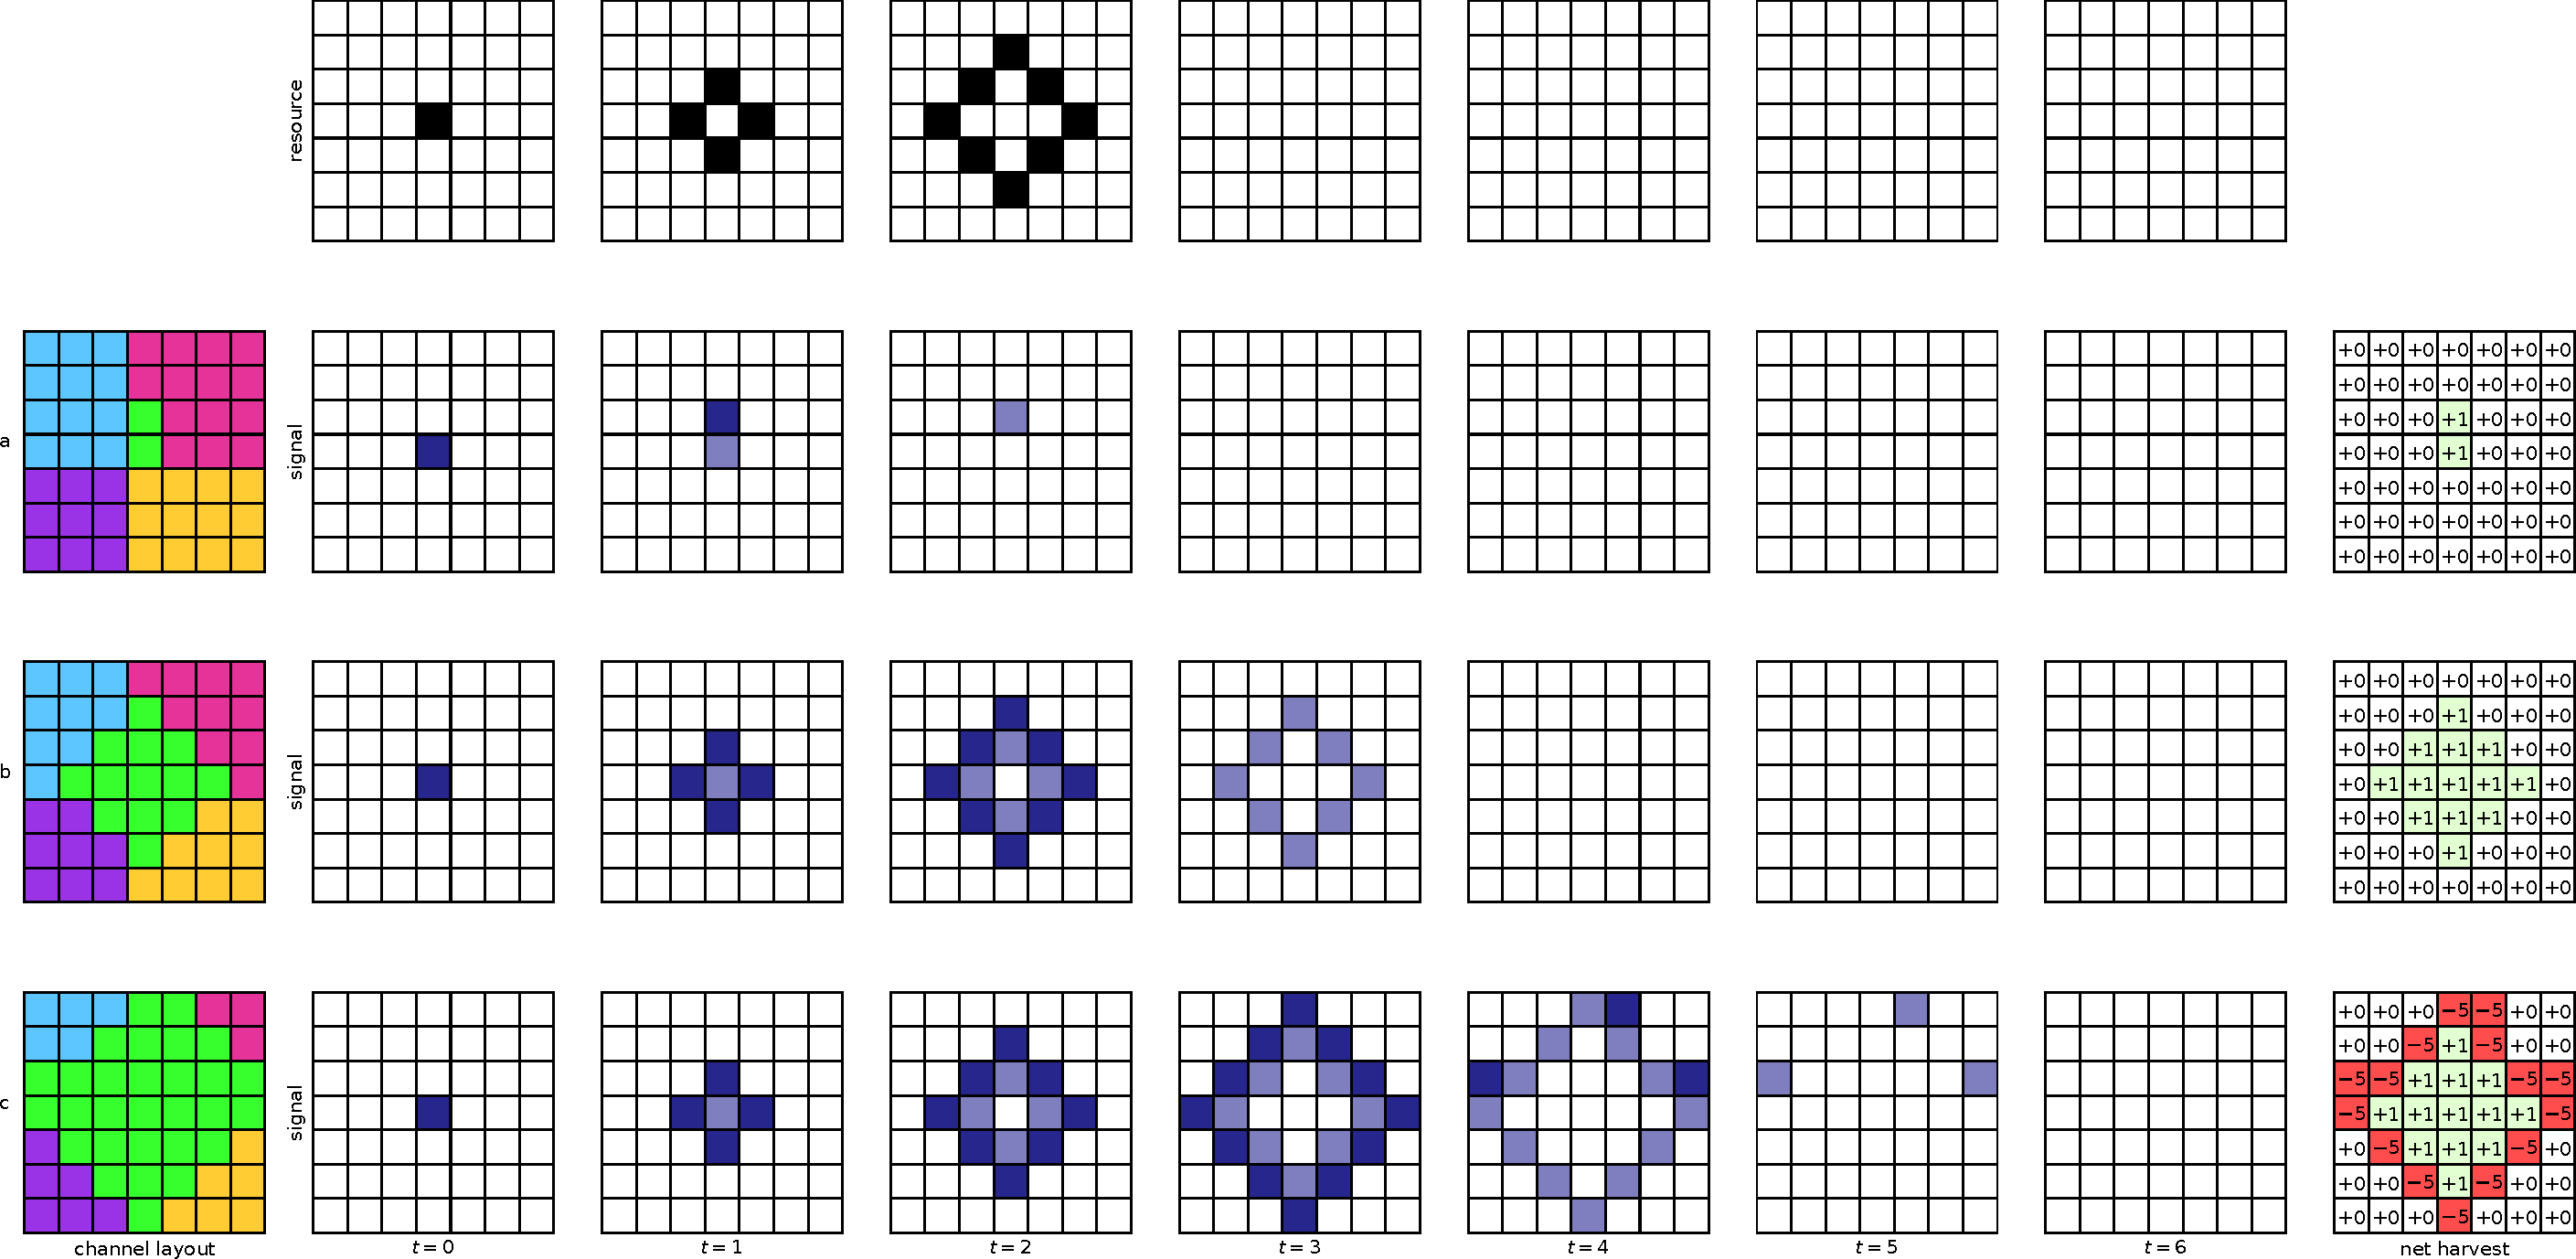
\includegraphics[width=2.0\columnwidth]{img/explanatory}
\caption{Activation-quiescence signaling, and net resource collection for three different channel configurations during a single resource wave events.}
\label{fig:explanatory}
\end{center}
\end{figure*}


DISHTINY allows cell-like organisms to replicate across a toroidal grid.
Over discrete timesteps (``updates''), the cells can collect a continuous-valued resource.
Once sufficient resource has been accrued, cells may pay $1.0$ resource to place a daughter cell on an adjoining tile of the toroidal grid (i.e., reproduce), replacing any existing cell already there.
Collected resource decays at a rate of 0.1\% per update, incentivizing its quick use.
As cells reproduce, they can choose to include offspring in the parent's cooperating ``signaling channel'' group or expel offspring to found a new cooperating ``signaling channel'' group.

As shown at the top of Figure \ref{fig:explanatory}, resource appears at a single point then spreads outwards update-by-update in a diamond-shaped wave. The expanding wave halts at a predefined limit.
Cells must enter an ``activated'' state to harvest resource as it passes overhead.
The cell at the starting position of a resource wave is automatically activated, and will propagate the activation signal to neighboring cells on the same signaling channel.
The newly activated cells, in turn, activate their own neighbors registered to the same signaling channel.
Neighbors registered to other signaling channels do not activate.
Each cell, after sending the activation signal, enters a temporary quiescent state.
In this manner, cells sharing a signaling channel track and harvest an expanding resource wave.
As shown Figure \ref{fig:explanatory}$a,b$, the rate of resource collection for a cell is determined by the size and shape of of its same-channel signaling network;
small or fragmented same-channel signaling networks will frequently miss out on resource as it passes by.

Resource waves have a limited extent.
Cells that activate outside the extent of a resource wave collect no resource.
A long quiescent period ensures that erroneously activated cells miss several subsequent opportunities to collect resource and therefore will tend to collect resource at a slower rate.
This erroneous activation scenario is depicted in Figure \ref{fig:explanatory}$c$.
In this manner, ``Goldilocks'' --- not to small and not too big --- signaling networks enjoy superior fitness.

Resource wave starting points (seeds) are tiled over the toroidal grid from a randomly chosen starting location such that the extents of the resource waves do not overlap.
All resource waves begin and proceed synchronously;
when they complete, the next resource waves are seeded.
This process provides efficient and spatially-uniform selection for ``Goldilocks'' same-channel signaling networks.

Cells control the size and shape of their same-channel signaling group through strategic reproduction.
Three choices are afforded: whether to reproduce at all, where among the four adjoining tiles of the toroidal grid to place their offspring, and whether the offspring should be registered to the parent's signaling channel or be given a random channel ID (in the range 1 to $2^{64} - 1$).
The probability of channel collision is miniscule: $60 \times 60 \times 2^{20}$ (the grid dimensions times the number of simulation updates) independent channel values will collide with probability less than $1 \times 10^{-9}$.
No guarantees are made about the uniqueness of a newly-generated channel ID, but chance collisions are rare.

Hierarchical levels are introduced into the system through multiple separate, but overlaid, instantiations of this resource wave/channel-signaling scheme.
We refer to each independent resource wave/channel-signaling system as a ``level.''
In some experimental treatments, we allowed two resource wave/channel-signaling levels, identified here as level one and level two.
On level one, resource waves extended a radius of two toroidal tiles.
On level two they extended a radius of six toroidal tiles.
On both levels, activated cells netted $+0.2$ resource from a resource wave, but did not collect any resource outside the extent of the resource wave.
Due to the different radii of resource waves on different levels, level one selects for small same-channel signaling networks and level two selects for large same-channel signaling networks.

Each cell contained a pair of separate channel IDs, the first for level one and the second for level two.
We kept these channel IDs hierarchically nested by constraining inheritance during reproduction.
Daughter cells could not inherit just the level-one channel ID, they could either
\begin{enumerate}
\item inherit both level-one and level-two channel ID,
\item inherit level-two channel ID but not level-one channel ID, or
\item inherit neither channel ID.
\end{enumerate}
Hierarchically nested channel IDs are analogous to a strict corporate organizational structure: all employees (i.e., cells) are members of one department (i.e., level-one channel network) and one corporation (i.e., level-two channel network) but no employee can be a member of two departments and no department can be a member of two corporations.
Figure \ref{fig:outcome_grids} depicts hierarchically nested channel states at the end of three evolutionary runs.

An evolutionary transition in individuality can readily be evaluated within the DISHTINY framework with respect to same-channel network groups.
In addition to a potentially functionally cooperative relationship, shared channel IDs --- which may only systematically arise through inheritance --- imply a close hereditary relationship.
Because new channel IDs arise first in a single cell, same-channel signaling networks are reproductively bottlenecked analogously to a "Staying Together" life cycle (rather than a "Coming Together" life cycle) \cite{staps2019emergence}.
This precludes chimeric groups, except for mutations arising from somatic reproduction and rare cases of channel ID collision.

To recognize an evolutionary transition in individuality, we can evaluate
\begin{enumerate}
\item whether cells with the same channel ID cooperate altruistically by assessing, for example, resource sharing, and
\item whether delegation of reproductive labor arises by assessing whether interior cells cede reproduction to those at the periphery.
\end{enumerate}
If cells sharing the same level-one channel fulfill these conditions, we would suppose that a first-level transition in individuality had occurred.
Likewise, if cells sharing the sharing the same level-two channel fulfill these conditions, we would suppose that a second-level transition in individuality had occurred.
Further, we can screen for the evolution of complex multicellularity by assessing cell-cell messaging, regulatory patterning, and functional differentiation between cells within the a same-channel signaling network \cite{knoll2011multiple}.

\subsection{Channel Group Life Cycle}

Mature same-channel resource collecting groups enjoy a considerable advantage over fledging propagules.
Because of the isometric scaling relationship between surface area and perimeter, cooperative same-channel resource collecting groups can marshal more resource at their periphery.
In addition, because of their greater surface area, mature same-channel resource collecting groups are able to seed resource-wave events and collect resource at a higher per-cell rate.

In order to ensure channel group turnover and facilitate channel group propagation, we impose a timed phase-out of somatic reproduction and resource wave harvests.
For each cell, we track a channel generation counter at each resource wave level.
At the genesis of a new channel group, these counters are set to zero.
Daughter cells that expand a channel group's soma are initialized to a counter value one greater than their parent.
Additionally, all channel generation counters are incremented every 512 updates to ensure that soma ages even in the absence of reproduction.
When a cell's channel generation counter reaches 1.5 times the wave radius of its level, it can no longer produce somatic daughter cells.
Then, after two additional counter steps, cells lose their ability to seed resource wave events and collect resource.
Thus, as channel groups age over time, their constituent cells lose the ability regenerate somatic tissue and then, soon after, to collect resource.
To prevent complete stagnation in the case where all cells' channel generation counters expire we provide a uniform inflow of $+0.0051$, sufficient for one reproduction approximately every thousand updates.

Interaction between nested channel groups produces a notable selective byproduct.
Because smaller, level-one channel groups tend to have intrinsically shorter lifespans, in order to achieve the full potential productive somatic lifespan of a larger, level-two channel group its constituent small channel groups must be intermittently regenerated.
Otherwise, the soma's capacity to seed resource-wave events and to collect resource will be prematurely lost once its constituent smaller, level-one channel groups expire.

This aging scheme's design ultimately stems from a desire
\begin{enumerate}
\item to facilitate evolution through regular turnover of emergent individuals and
\item to scaffold workable propagation for primitive cellular strategies while furnishing opportunities for more sophisticated adaptations to the imposed life cycle constraints.
\end{enumerate}
However, in some sense the aging scheme is heavy-handed, in effect enforcing rather than enabling a birth-death life cycle.
The evolutionary basis of aging and mortality --- in particular, the possibility of intrinsic evolutionary adaptations promoting these phenomena in addition to extrinsic factors  --- remains an active topic of scientific discussion [lotsa citations TODO].
In future work, we are interested in evaluating the outcomes of relaxing constraints of this aging scheme under different evolutionary conditions (such as cosmic ray mutations or irregular population structure) in light of theory attributing mortality and aging to evolvability, mutational accumulation, and costly somatic maintenance [lotsa citations TODO].

\subsection{Cell-Level Organisms}

\begin{figure}
\begin{center}

\hspace*{\fill}%
\begin{minipage}[t]{\columnwidth}
\centering
\vspace{0pt} % for alignment
\begin{subfigure}[b]{\textwidth}
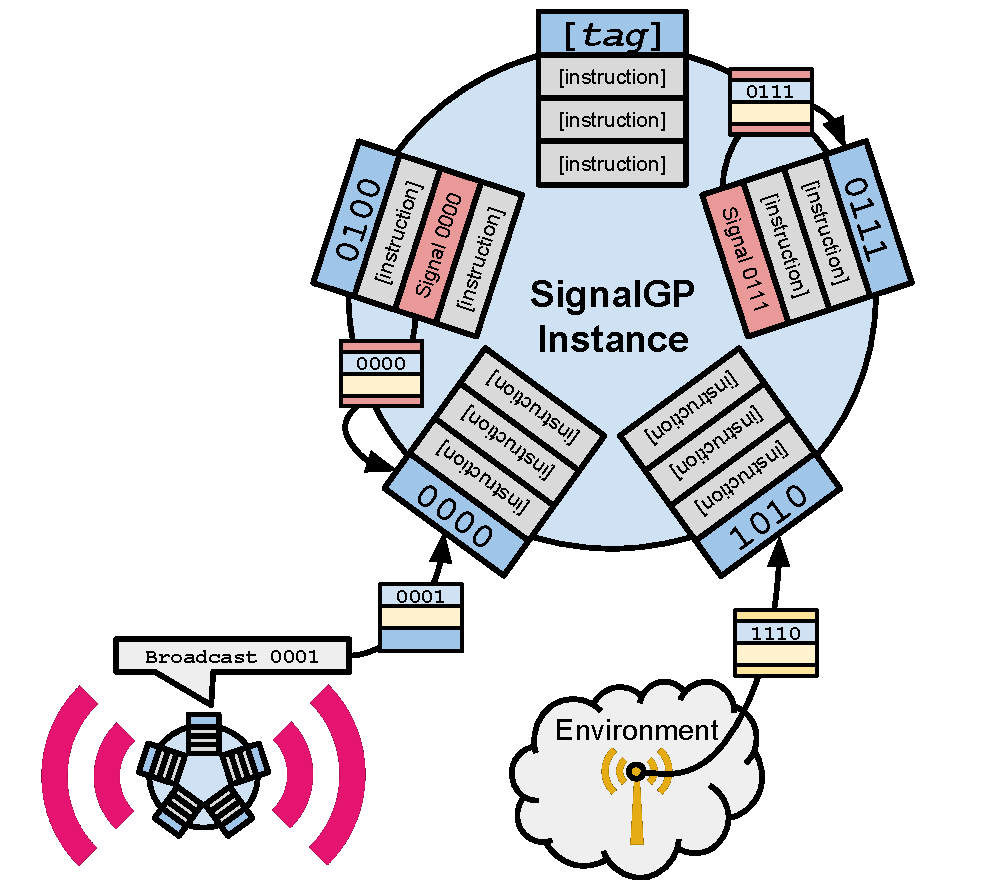
\includegraphics[width=\textwidth]{img/signalgp-cartoon}%
\caption{
A cartoon overview of a single SignalGP instance.
SignalGP program modules execute pseudo-concurrently in response to tagged signals, which can originate internally, from the environment, or from other agents.
}
\label{fig:signalgp-cartoon}
\end{subfigure}
\end{minipage}%
\hspace*{\fill}

\hspace*{\fill}%
\begin{minipage}[t]{\columnwidth}
\centering
\vspace{0pt} % for alignment
\begin{subfigure}[b]{\textwidth}
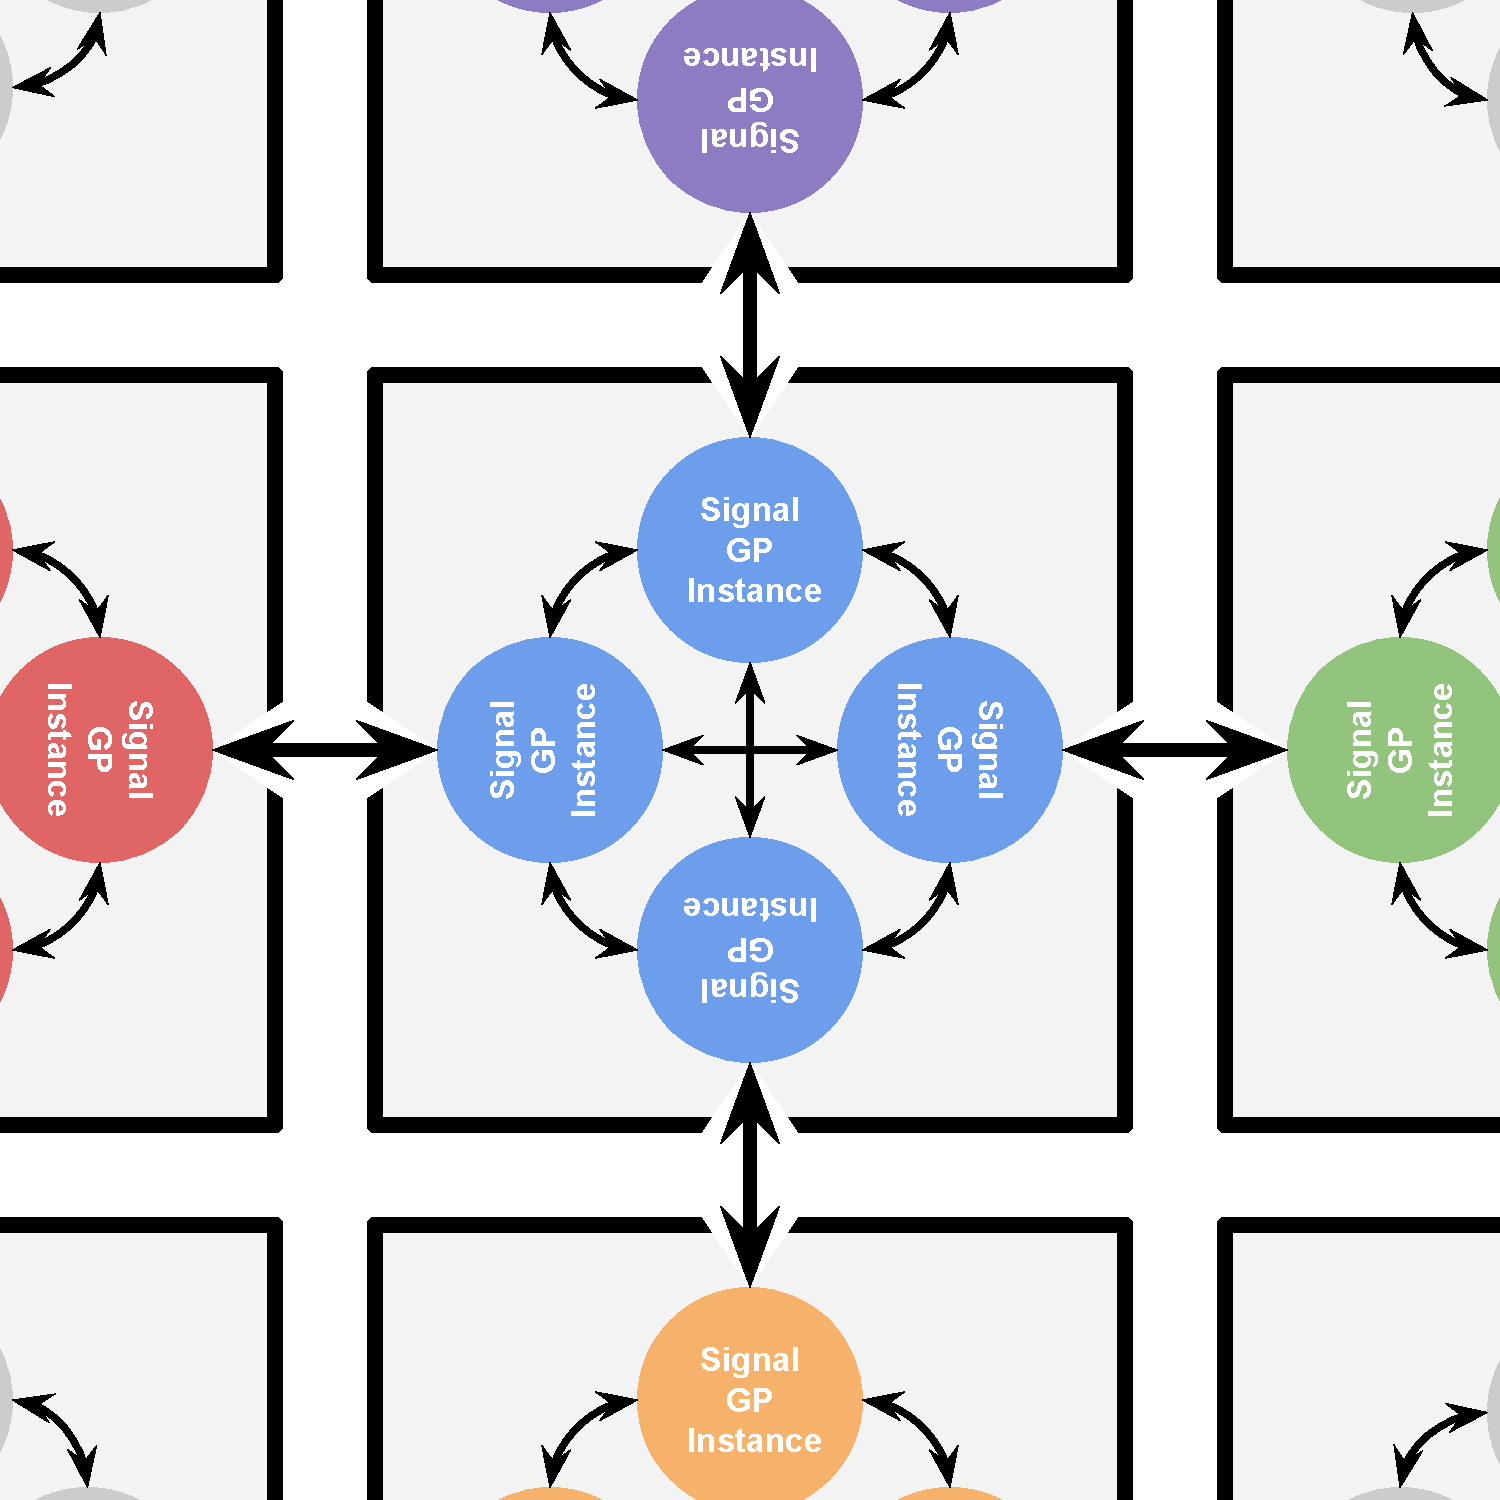
\includegraphics[width=\textwidth]{img/dishtinygp-cartoon}
\caption{
A cartoon overview of how individual SignalGP instances are organized into DISHTINY cells.
% Each cell contains four independent SignalGP instances.
% The same genetic program is mirrored across all four SignalGP instances, but each instance executes independently.
Within each DISHTINY cell, each of four independent instances senses environmental state, receives intercellular messages, and determines cell behavior with respect to a single cardinal direction.
All four instances sense non-directional environmental cues and non-directional actions may be taken by any instance.
Instances within a cell communicate via intracellular messaging.
}
\label{fig:dishtinygp-cartoon}
\end{subfigure}
\end{minipage}%
\hspace*{\fill}


\caption{
Schematic illustrations of how individual SignalGP instances function and how individual SignalGP instances are organized into DISHTINY cells.
Figure \ref{fig:signalgp-cartoon} provided courtesy Alexander Lalejini.
}
\label{fig:signalgp-dishtinygp}
\end{center}
\end{figure}


We performed our experiments using cell-level digital organisms controlled by evolving SignalGP programs.
SignalGP is genetic programming framework designed around the event-driven programming paradigm \cite{lalejini2018evolving}.
SignalGP programs are collections of independent procedural functions, each equipped with a bit-string tag.
A function is triggered by a signal with affinity that maximally and sufficiently matches its tag.
(A binding threshold of 0.1 was used in these experiments).
Signals may be generated by the environment, received as messages from other agents, or triggered internally by function execution.
Signals, and the ensuing chains of procedural execution they give rise to, are processed pseudo-concurrently by 24 virtual CPU cores.
Figure \ref{fig:signalgp-dishtinygp}(TODO a) schematically depicts a single SignalGP instance.

In this work, we introduce a regulatory extension to the SignalGP system.
During runtime, instructions may increase or decrease each tagged function's intrinsic tendency to match with --- and activate in response to --- tagged queries.
Intrinsic tag-to-tag match distances $m$ are modulated by a regulator value $r$ (baseline, 1.0) to become $r + r \times m$.
This scheme allows a function to be upregulated such that every query activates that function (e.g., $r = 0$) or no query activates that function (e.g., $r = \texttt{inf}$).
These regulation settings are heritable during reproduction but automatically decay after a number of updates determined when they are set.

To allow cells to protect themselves form potentially antagonistic interactions with their neighbors, we filter intercellular messages through a tag-matching membrane.
At runtime, cells can embed tags in this membrane that either admit or repel incoming messages.
Messages that do not match with a membrane tag are repelled.
A message, for example, that would activate a SignalGP function containing an apoptosis instruction could be rejected while other messages are accepted.
Tags embedded in this membrane automatically decay and may also be regulated.
We also filter messages between hardware instances within the same cell through a tag-matching membrane, but the default behavior for messages with unmatched tags is admission rather than rejection.

Previous work evolving digital organisms in grid-based problem domains has relied on a single computational instance which designates a direction to act in via an explicit cardinal ``facing'' state or output \cite{goldsby2014evolutionary, goldsby2018serendipitous, grabowski2010early, biswas2014causes, lalejini2018evolving}.
Under this paradigm, a large portion of genotype space encodes behaviors that are intrinsically asymmetrical with respect to absolute or relative (depending on implementation) cardinal direction.
However, in grid-based tasks, directional phenotypic symmetry is generally advantageous.
That is --- in the absence of a polarizing external stimulus --- successful agents generally behave uniformly with respect to each cardinal direction of the grid.
In this work, each cell employs four instances of SignalGP hardware: one ``facing'' each cardinal direction.
These computational instances all execute the same SignalGP program but are otherwise decoupled and may follow independent chains of execution and develop independent regulatory states.
These instances execute round robin step-by-step in an order that is randomly drawn at the outset of each update.

Genetic encodings that exploit problem-domain symmetries are known to promote evolvability and --- ultimately --- evolved solution quality \cite{clune2011performance, cheney2014unshackling}.
We submit that this directional hardware replication protocol likely increases the fraction of genotype space that encodes cardinally-symmetric phenotypes and therefore better facilitates the evolution of high-fitness phenotypes.
In further work, we look forward to exploring the evolvability and solution quality implications of this new approach.

The single SignalGP program that is mirrored across the cell's computational instances represents the cell's genome.
Mutation, with standard SignalGP mutation parameters as in \cite{lalejini2018evolving}, is applied to 1\% of daughter cells at birth.
In addition, genomes encode the bitstrings associated with environmental events.
These bitstrings evolve at a per-bit mutation rate equivalent to the bitstring labels of SignalGP functions.

Instances within a cell may send intracellular messages to one another or intercellular messages to a neighboring cell.
Intercellular messages are received by the SignalGP instance that faces the sending cell.
Figure \ref{fig:signalgp-dishtinygp}(TODO b) schematically depicts the configuration of the four SignalGP instances that constitute a single DISHTINY cell as well as the instances of neighboring cells that receive extracellular messages from the focal cell.

We performed our experiments on a traditional 60-by-60 toroidal grid, supporting a population of at most 3600 individual cells.
As each cell contained four SignalGP instances, our simulations encompassed up to 14,400 virtual CPUs with up to 345,600 virtual cores.
In order to reduce the computational burden of our experiment, we intermittently advanced the virtual CPUs.
Every four updates, virtual CPUs were advanced 16 cycles.
Intracellular messages were delivered immediately after they were generated.
Intercellular messages, cached in first-in first-out inboxes with maximum capacity 16, were retrieved every four updates.
Event-driven environmental cues and Accrued cell actions were dispatched every eight updates.

Evolving programs employed combinations of the event-driven environmental cues, procedural instruction-based sensors, and procedural instruction-based actuators detailed in the following two subsections.

\subsection{Instruction Library}

In addition to the generic arithmetic, logic, and program flow instructions in the default SignalGP instruction set, which is laid out in \cite{lalejini2018evolving}, we define the following instructions.
Instructions that involve an extracellular neighbor default to the cell that the executing SignalGP instance is facing.

\begin{itemize}
\item \textbf{RNG Draw}
Draw a random value between 0.0 and 1.0 from random number generator and store result in a register.
\item \textbf{Send/Broadcast Intracellular Message}
Send a message to a single other SignalGP instance within the cell or to all SignalGP instances (except the executing instance) within the current cell.
\item \textbf{Set Stockpile Reserve}
Mark twice the amount of resource as ineligible for sharing.
The amount may be modified by a register-based argument.
\item \textbf{Activate/Deactivate Intercellular Inbox}
Mark or unmark the intercellular inbox in a particular direction to refuse incoming messages.
At cell birth, the inbox is deactivated.
\item \textbf{Share Resource}
Send a proportion of the cell's stockpiled resource to a neighboring cell.
One instruction defaults to sending a large proportion of available resource (50\%) to the neighboring cell.
A second instruction defaults to sending a small proportion of available resource (5\%) to the neighboring cell.
The proportion of available resource can be adjusted by a register-based argument.
\item \textbf{Accept/Decline Sharing}
Mark the cell to decline resource sent by neighbors.
Declined resource is retained by the sending cell (with no resource lost).
Regardless of this instruction, cells with negative resource stockpiles automatically decline shared resource.
At birth, the cell is marked to accept sharing.
\item \textbf{Send/Broadcast Intercellular Message}
Send a message to a single cellular neighbor or to all cellular neighbors.
\item \textbf{Reproduce}
Attempt to spawn a child cell in a particular direction, paid for out of the parent cell's resource stockpile.
If sufficient resource is not available in the cell's stockpile, no resource is action is taken.
Variants of this instruction are defined for each channel ID inheritance level: from endowing the daughter cell with the parental channel IDs across all levels, to endowing the daughter cell with a new level-one channel ID but the parent's level-two channel ID, to endowing the daughter cell with all-new channel IDs.
If a channel generation counter limit has been reached, reproduction is simply attempted at the next highest level; even with channel generation counters maxed out, cells may generate offspring with all-new channel IDs.
\item \textbf{Pause Reproduction}
Pause cellular reproduction in a single direction for the remainder of the current update and for the entire next update.
Variants of this instruction pause reproduction at a certain wave/channel-signaling level or across all channel ID inheritance levels.
\item \textbf{Increase Channel Generation Counter}
Increases the cell's channel generation counter by one.
The amount the cell's generation counter is increased by can be adjusted by register-based argument.
\item \textbf{Apoptosis}
The cell is killed at the end of the current update.
Two variants are defined.
Under the conplete variant, the cell's channel ID partial and complete
\item \textbf{Designate/Revoke Heir} On apoptosis, 50\% of the reproduction cost to establish a cell and the dying cell's own stockpile amount split evenly among neighboring cells that are designated at the time of death.
These instructions mark or un-mark a neighbor as a heir.
\item \textbf{Query Own Stockpile}
Sets a designated register to the amount of resource present in the cell's stockpile.
\item \textbf{Query Own Channel Generation Counter} -Lev
This instruction sets a designated register to the value of the cell's channel generation counter.
A variant of this instruction is provided for each wave/channel-signaling level.
\item \textbf{Query ``Is Neighbor Live?''}
This instruction sets a designated register to 1 if the neighboring tile contains a live cell and 0 otherwise.
\item \textbf{Query ``Is Neighbor Channel Set?''}
This instruction sets a designated register to 1 if the neighboring tile contains active channel IDs and 0 otherwise.
\item \textbf{Query ``Is Neighbor My Cellular Child?''}
This instruction sets a designated register to 1 if the neighboring cell is the daughter of the querying cell and 0 otherwise.
\item \textbf{Query ``Is Neighbor My Cellular Parent?''}
This instruction sets a designated register to 1 if the neighboring cell is the parent of the querying cell and 0 otherwise.
\item \textbf{Query ``Does Neighbor's Channel ID Match Mine?''}
This instruction sets a designated register to 1 if the neighboring cell has the same channel ID as the querying cell and 0 otherwise.
A variant of this instruction is provided for each wave/channel-signaling level.
\item \textbf{Query ``Does Neighbor's Channel ID Descend From Mine?''}
This instruction sets a designated register to 1 if the neighboring cell's highest-level channel ID is different from the querying cell's highest-level channel ID, but is descended from the querying cell's channel ID.
This instruction allows a querying cell to sense whether its neighbor is a member of a same-channel group that is a propagule of the querying cell's same-channel group.
\item \textbf{Query ``Does My Channel ID Descend From Neighbor's?''}
This instruction sets a designated register to 1 if the querying cell's highest-level channel ID is different from the neighboring cell's highest-level channel ID, but is descended from the neighboring cell's channel ID.
\item \textbf{Query Neighbor's Channel ID}
This instruction sets a designated register to the neighbor's channel ID.
\item \textbf{Query Neighbor's Stockpile}
This instruction sets a designated register to the amount of resource present in the neighbor's stockpile.
\end{itemize}

To ensure a founding crop of viable individuals, apoptosis and program flow instructions in the initial randomly-generated population were replaced with no-op instructions.
However, these instructions were allowed to mutate in to genomes freely once evolutionary runs began.

\subsection{Event Library}

The activating affinity of each event is set at the outset of each experiment using a pseudo random number generator.

\begin{itemize}
\item \textbf{On Update}
This event is triggered at the outset of each simulation update.
\item \textbf{Facing Cellular Child}
This event is triggered at the outset of an update if the SignalGP instance is facing a neighboring cell that is the querying cell's daughter.
\item \textbf{Stockpile Debt}
This event is triggered at the outset of an update if the amount of resource in a cell's stockpile is negative.
\item \textbf{Neighbor's Channel ID Matches Mine} defined per level
This event is triggered at the outset of an update if a SignalGP instance is facing a neighbor cell that shares its channel ID.
A different event is provided for each resource wave/channel-signaling level.
\item \textbf{Neighbor's Channel ID Descends From Mine}
This event is triggered at the outset of an update if the neighboring cell's highest-level channel ID is different from the querying cell's highest-level channel ID, but is descended from the querying cell's channel ID.
This event allows a querying cell to sense whether its neighbor is a member of a same-channel group that is a propagule of the querying cell's same-channel group.
\end{itemize}

\subsection{Treatments}

In this work, we screened replicates conducted under combinations of two experimental conditions:
\begin{enumerate}
\item flat versus nested hierarchical resource wave/channel-signaling levels and
\item cooperative versus independent resource collection.
\end{enumerate}

The first experimental manipulation explores the effects of hierarchical nesting of kin-sensing and/or functional cooperation.
The second manipulation explores the effects of functional cooperation.

\begin{table*}[!htbp]
\begin{center}

\begin{filecontents*}{productivity.csv}
Measure,Nested,Flat,Even
Per-cell-update resource inflow,$0.0178 \pm 0.0010$,$0.0145 \pm 0.0008$,$0.0175 \pm 0$
Per-cell-update cell reproduction,$0.0117 \pm 0.0023$,$0.0094 \pm 0.0018$,$0.0113 \pm 0.0018$
\end{filecontents*}

\begin{tabular}{l|c|c|c}%
\bfseries Measure
  & \bfseries Even
  & \bfseries Flat
  & \bfseries Nested
\csvreader[head to column names]{productivity.csv}{}
{\\\hline\Measure
  & \Nested
  & \Flat
  & \Even
}
\end{tabular}

\caption{
Observed productivity at epoch 1 (mean $\pm$ S.D.)
}
\label{tab:productivity}
\end{center}
\end{table*}


To enact the first manipulation, we compared the nested hierarchical resource wave/channel-signaling scheme described above with a single-level scheme with waves extending six toroidal tiles.
We also increased the resource wave reward to $+0.6$ to approximately match the observed resource inflow rate of the nested scheme.
To enact the second manipulation, we removed the resource wave reward and increased the uniform resource inflow rate to $+0.0175$ in order to approximately match the net inflow rate under the dual-level wave-based scheme.
Table \ref{tab:productivity} reports productivity observed under these different conditions.

We mix and match these experimental manipulations in three treatments:
\begin{enumerate}
\item two levels with wave-based resource (``nested''),
\item one level with wave-based resource (``flat''), and
\item two levels with even resource, kin-sensing (``even'').
\end{enumerate}

\begin{figure*}[!htbp]
\begin{center}

\begin{filecontents*}{systematics.csv}
Measure,NestedShort,FlatShort,EvenShort,NestedLong,FlatLong,EvenLong
Replicate count,40,40,40,37,40,39
Cellular generations elapsed,$953 \pm 563$,$1140 \pm 697$,$935 \pm 636$,$4635 \pm 3077$,$5869 \pm 3246$,$4628 \pm 3274$
Level 1 generations elapsed,$566 \pm  637$,$127 \pm 68$,$592 \pm 553$,$2637 \pm 2933$,$654 \pm 353$,$2908 \pm 2768$
Level 2 generations elapsed,$121 \pm  85$,N/A,$117 \pm  99$,$546 \pm 349$,N/A,$526 \pm  352$
Phylogenetic depth,$14 \pm 6$,$14 \pm  6$,$15 \pm 8$,$54 \pm 31$,$55 \pm 26$,$60 \pm 44$
Coalescent replicates,58.5\%,77.5\%,62.5\%,94.6\%,97.5\%,92.3\%
\end{filecontents*}

\begin{tabular}{l|c|c|c|c|c|c}%
&\multicolumn{3}{c|}{Update 262144}
&\multicolumn{3}{c}{Update 1048576}\\
\bfseries Measure
  & \bfseries Nested
  & \bfseries Flat
  & \bfseries Even
  & \bfseries Nested
  & \bfseries Flat
  & \bfseries Even
\csvreader[head to column names]{systematics.csv}{}
{\\\hline\Measure
  & \NestedShort
  & \FlatShort
  & \EvenShort
  & \NestedLong
  & \FlatLong
  & \EvenLong
}
\end{tabular}

\caption{
Systematics information TODO
}
\label{fig:systematics}
\end{center}
\end{figure*}


We ran 40 replicates under each treatment condition.
All replicates ran to at least 262144 updates, and all comparisons between or within treatments are conducted at this time point.
However, some replicates were able to run to 1048576 updates during the available compute time.
Reported case studies of individual replicates are

Table \ref{tab:systematics} reports the systematics outcomes observed under each treatment.

\subsection{Implementation}

We implemented our experimental system using the Empirical library for scientific software development in C++, available at \url{https://github.com/devosoft/Empirical}.
The code used to perform and analyze our experiments, our figures, data from our experiments, and a live in-browser demo of our system is available via the Open Science Framework at \url{https://osf.io/g58xk/}.
Most replicates finished within a day, but some took up to a week to complete.
